\subsection{Limitaciones de los sensores}

\subsubsection{Limitación de lectura del potenciómetro}

El potenciómetro se comporta como un divisor resistivo variable, por lo que la medición que se realiza con el microcontrolador resulta en una tensión entre $V_{\min} = \qty{0}{\V}$ y $V_{\max} = \qty{5}{\V}$, dependiendo de la posición de la perilla. El microcontrolador, un Arduino UNO, realiza la medición utilizando un conversor analógico-digital de $N = 10$ bits de resolución, lo que resulta en 1024 símbolos posibles, equidistantes en tensión. Por lo tanto, la resolución mínima de lectura del potenciómetro estará dada por
\begin{equation*}
    \Delta V = \frac{V_{\max} - V_{\min}}{2^N} = \frac{\qty{5}{\V}}{1024} \approx \qty{5}{\mV}.
\end{equation*}

Si realizamos un mapeo del rango de tensiones a un rango de ángulos entre \qty{-90}{\degree} y \qty{90}{\degree}, entonces la resolución angular será dada por
\begin{equation*}
    \Delta \theta = \frac{\theta_{\max} - \theta_{\min}}{2^N} = \frac{\qty{180}{\degree}}{1024} \approx \qty{0.18}{\degree}.
\end{equation*}

Para calcular el tiempo requerido para realizar una medición, se realizaron 100 mediciones consecutivas del ADC y se promedió el tiempo de cada una. El valor obtenido fue de \qty{112}{\us}.

Entonces, con la estrategia del potenciómetro y el conversor analógico-digital del microcontrolador se pueden establecer ángulos de referencia con una resolución angular de \qty{0.18}{\degree}, y el tiempo para realizar una medición es de \qty{112}{\us}. Esto es más que apropiado para el diseño de un lazo de control del \emph{ball-and-beam}.

\subsubsection{Limitación de lectura del sensor de distancia}

El sensor de distancia funciona enviando un pulso sonoro cuando se inicia la medición, para luego informar la cantidad de tiempo transcurrido hasta que la señal reflejada en un obstáculo regresa al sensor. A partir de conocer la velocidad del sonido en el aire, puede calcularse la distancia a la que se encuentra el obstáculo. La resolución temporal que provee la biblioteca \verb|NewPing.h| es de $\Delta t = \qty{4}{\us}$ para el tiempo de vuelo total, ya que utiliza un temporizador del microcontrolador con dicha resolución. Dado que la expresión que relaciona el tiempo de vuelo con la distancia es
\begin{equation*}
    d = \frac{v t}{2},
\end{equation*}
con $v$ la velocidad del sonido en el aire, entonces la resolución en distancia asociada será, teóricamente,
\begin{equation}
    \label{eq:dist-tiempo-errores}
    \Delta d = \frac{v}{2} \Delta t \approx \qty{0.7}{\mm},
\end{equation}
usando un valor estándar de $v = \qty{340}{\m\per\s}$.

Sin embargo, los valores de distancia y de tiempo provistos por la biblioteca son artificialmente más precisos que los que se obtiene en la realidad. La hoja de datos del sensor indica que su resolución en distancia es del orden de los \qty{3}{\mm}, una precisión considerablemente peor. Por lo tanto, se toma a este valor como la resolución real del dispositivo, la cual se considerará para el control del \emph{ball-and-beam}. Despejando de \eqref{eq:dist-tiempo-errores}, la mínima resolución temporal real será de aproximadamente \qty{18}{\us}.

El tiempo que se demora en realizar una medición depende de la distancia al objeto. Se realizaron mediciones experimentales del tiempo de medición, variando la distancia de medición para obtener un rango. En la biblioteca se estableció una distancia máxima de \qty{50}{\cm}, para limitar el tiempo de espera en caso de que el obstáculo se encuentre demasiado lejos. Este valor es más que suficiente para controlar el \emph{ball-and-beam}, ya que la varilla tiene una longitud menor a \qty{50}{\cm}. Las mediciones realizadas sitúan al tiempo de medición entre los \qty{2.4}{\ms} para obstáculos extremadamente cercanos al sensor, y los \qty{5.2}{\ms} para obstáculos muy lejanos donde entra en juego la limitación de los \qty{50}{\cm}. Se considerará entonces que el sensor demora \qty{5.2}{\ms} en realizar una medición, adoptando el peor caso.

En resumen, con el sensor de distancia se podrá medir la posición del carro con una resolución de \qty{3}{\mm}, más que suficiente para el diseño del lazo de control sobre una barra de longitud \qty{30}{\cm}. El tiempo para tomar una medición es considerable pudiendo llegar a los \qty{5.2}{\ms}, pero aún permite margen para realizar un control a \qty{50}{\Hz}, que permite hasta \qty{20}{\ms} para cómputo por cada iteración.

% TODO: Relación de la velocidad del sonido con la temperatura (aparentemente casi no varía con la presión).

\subsubsection{Limitación de lectura de la unidad de medición inercial}

Para la estimación del ángulo de la barra se utiliza una unidad de medición inercial (IMU) modelo MPU6050. La misma cuenta con un acelerómetro de 3 ejes que mide la aceleración lineal en cada uno de los ejes cartesianos, y un giróscopo que mide la velocidad angular alrededor de cada uno de dichos ejes. El acelerómetro provee una medición insesgada del ángulo pero muy ruidosa, mientras que el giróscopo permite medir la dinámica angular de alta frecuencia con muy bajo ruido pero a costa de una deriva temporal (\emph{drift}). Por lo tanto, la estimación se realiza a partir de ambos sensores, combinados utilizando un filtro complementario, que esencialmente consta de un pasa bajos aplicado al acelerómetro ---eliminando el ruido de alta frecuencia---, y un pasa altos aplicado al giróscopo ---eliminando la deriva---.

Dado que el giróscopo captura la dinámica del movimiento angular, para considerar la resolución de la IMU en reposo solo será necesario considerar al acelerómetro. El acelerómetro se encuentra configurado para devolver mediciones con un fondo de escala de \qty{78.5}{\m\per\s\squared} (8 gravedades). Su hoja de datos indica que la resolución en este caso se corresponde con 4096 LSB por gravedad. Por lo tanto, la mínima unidad discernible en cada eje será de
$$\Delta a = \frac{1}{4096 \, \mathrm{LSB}/g} = \num{244e-6} \, g = \qty{2.4e-3}{\m\per\s\squared}.$$

Por trigonometría, puede utilizarse la medición del acelerómetro para medir ángulos respecto de la vertical, ya que en dicha dirección se espera tener siempre una aceleración igual a una gravedad. Suponiendo que el acelerómetro gira siempre alrededor de un único eje ---de aquí en adelante, el eje $x$---, y que hay otro eje ---el eje $z$---, que apunta en dirección vertical para ángulo cero, entonces el ángulo de giro puede calcularse a como
$$\theta = \tan^{-1}\left(\frac{a_y}{a_z}\right).$$

Para ángulos pequeños, donde $a_z \approx g$, podemos aproximar
$$\theta \approx \frac{a_y}{g},$$
por lo que la resolución teórica estará dada por
$$\Delta \theta = \frac{\Delta a}{g} = \qty{244e-6}{\radian} = \qty{0.014}{\degree}.$$

Sin embargo, como se mencionó, las mediciones provenientes del acelerómetro son altamente ruidosas. Se midió experimentalmente el ángulo obtenido desde el acelerómetro para un ángulo estático de \qty{0}{\degree}. Se observa en la Figura~\ref{fig:ruido-acel} que la señal tiene un ruido de amplitud aproximada de \qty{0.3}{\degree}. Por lo tanto, será difícil distinguir ángulos menores a los \qty{0.3}{\deg}, y no se podrá aprovechar toda la resolución antes calculada de \qty{0.014}{\degree}. Por lo tanto, se considera que la mínima resolución obtenible para la medición de ángulos utilizando solo el acelerómetro será de \qty{0.3}{\degree}. Sin embargo, este valor es más que apropiado para el control que se desea realizar, más aún si se realiza un filtrado complementario que capture la dinámica con mejor resolución y elimine el ruido de alta frecuencia obtenido.

\begin{figure}
    \centering
    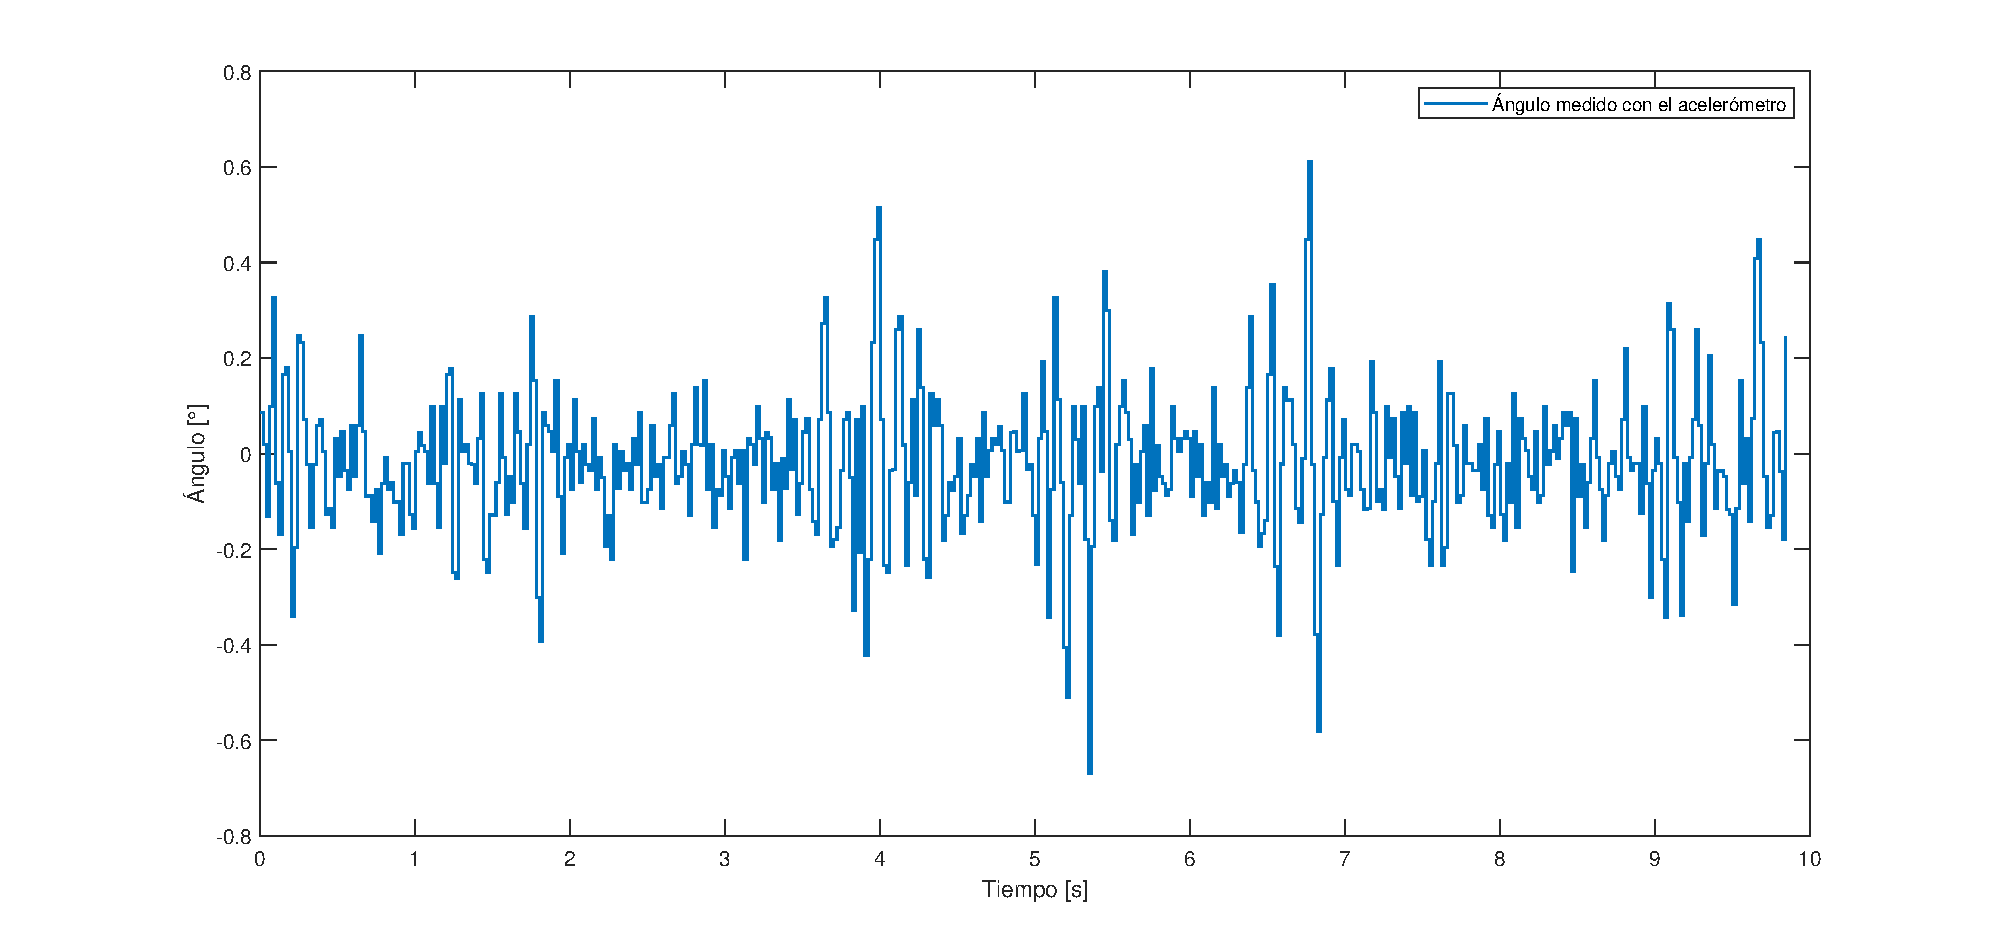
\includegraphics[width=0.8\linewidth]{resol_acelerometro}
    \caption{Ángulo estimado en condiciones estáticas utilizando solo el acelerómetro.}
    \label{fig:ruido-acel}
\end{figure}

Para obtener el tiempo necesario para realizar una lectura de la IMU, se leyó el sensor 100 veces en forma consecutiva y se promedió el tiempo de todas ellas. Se obtuvo un tiempo promedio de \qty{3.06}{\ms} para una lectura.

% vim: ts=4 sts=4 sw=4 et lbr
